\section{Vue globale}

\begin{figure}[H]
  \caption{Architecture trois tiers}
  \centering
  \vspace*{0.5cm}
  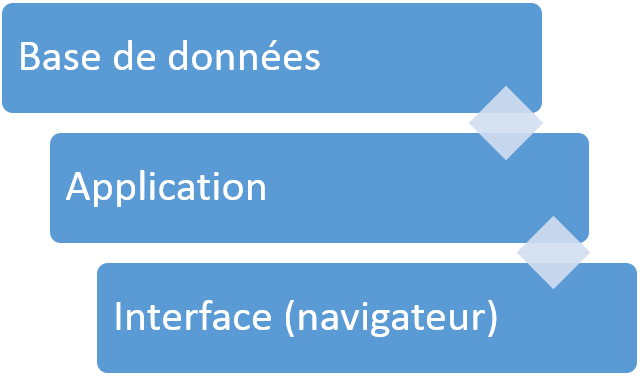
\includegraphics[width=10cm]{implem_1.png}
\end{figure}
Couche de présentation – Premier niveau : Interface web par navigateur.\\
Il s’agit d’une interface web qui permet au client d’interagir avec la solution.\\
Cette couche a pour vocation de relayer les requêtes de l’utilisateur à destination de la couche métier mais aussi d’afficher les informations envoyées par la couche métier à celle-ci. On parle donc d’une interface homme machine.\\
La couche de présentation sera disponible au travers d’une interface web utilisant le framework Django, adoptant un modèle MVT (Modèle-Vue-Template) :\\
\begin{figure}[H]
  \caption{Modèle MVT}
  \centering
  \vspace*{0.5cm}
  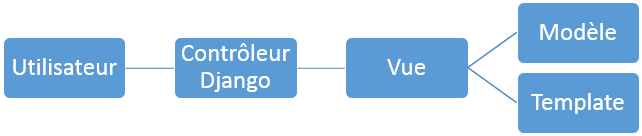
\includegraphics[width=15cm]{implem_2.png}
\end{figure}
\noindent
Couche métier – Second niveau : Application et interpréteur de données.\\
L’application aura pour vocation d’interpréter les données envoyées par la couche d’accès aux données, de les rendre intelligibles, et de les transmettre à la couche de présentation.\\
Elle permettra aussi de communiquer les requêtes de la couche présentation à la couche d’accès aux données en effectuant le travail inverse, transformer une requête simple émise par le premier niveau en langage complexe compréhensible par le troisième niveau. En résumé, la couche métier a pour objectif le traitement des données qui transitent entre le premier niveau et le troisième niveau et de s’assurer que les données soient compréhensibles pour les niveaux en les transformant au format adéquat.\\
Couche d’accès aux données – Troisième niveau : Basse de donnée et corrélation
Cette couche a pour but de stocker des données et de les rendre facilement accessibles pour la couche métier.  Les données stockées seront sauvegardées et/ou archivées parce qu’elles sont destinées à rester de manière définitive dans la base. Cette couche est aussi capable de recevoir des ordres interprétés par la couche métier.\\
\section{Couches applicatives}

\begin{figure}[H]
  \caption{Couche applicative}
  \centering
  \vspace*{0.5cm}
  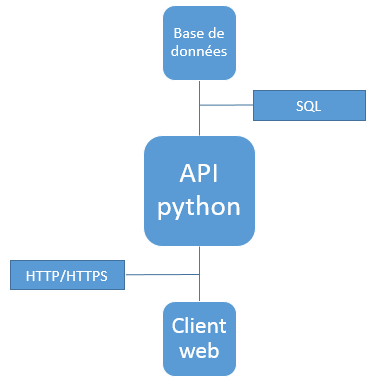
\includegraphics[width=10cm]{implem_3.png}
\end{figure}
